\documentclass[25pt, a2papper, portrait]{tikzposter}
\usepackage[utf8]{inputenc}

\usepackage{blindtext}
\usepackage{comment}
\usepackage{url}

\title{Deep: optimizer with embedded interpreter}
\author{A.~V.~Svichkarev, K.~N.~Kozlov}
\institute{System biology and bioinformatics lab, IAMM,\\
    Peter the Great St.Petersburg Polytechnic University,
    St.Petersburg, Russia\\[0.5cm]
    email: \url{tolik0393@bionet.nsc.ru}
}

\usetheme{Envelope}

\begin{document}

\maketitle


\begin{columns}
    \column{0.6}
    \block{Differential Evolution}
    {
        \begin{tikzfigure}
            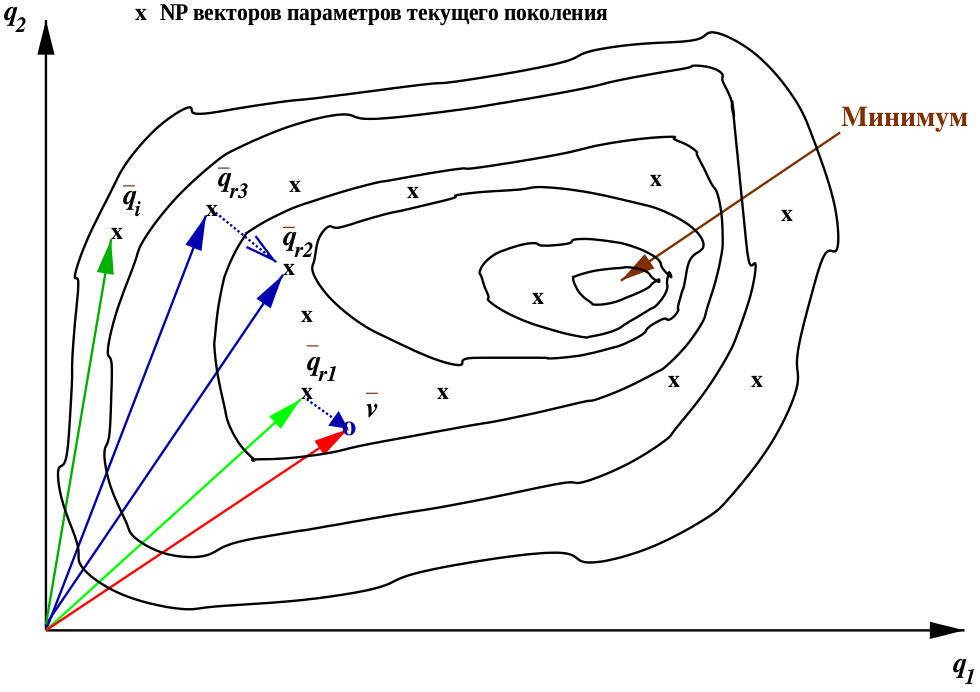
\includegraphics[width=0.45\textwidth]{images/DE}
        \end{tikzfigure}
    }

    \column{0.4}
    \block{Introduction}{
        The problem of parameter estimation
        for data-driven models in systems biology
        is challenging due to the diversity
        of biomedical applications and
        the necessity to treat large sets of
        heterogeneous data in specialized formats.
        These tasks usually require
        specialized computer environment
        and interpreted language for
        mathematical modelling.
        However, this approach makes
        numerical estimation of parameters
        of a mathematical model extremely
        computationally expensive.
    }
    \block{Problem}{
        Here we propose
        an enhancement to the
        Differential Evolution Entirely Parallel (DEEP) method
        developed recently.
        Our approach reduces the
        communication bottleneck
        between DEEP and objective function
        that describes the deviation
        of model solution
        from the data.
        An interpreter needed to
        calculate model solution
        is embedded into
        DEEP that uses
        master-slave architecture.
        A master process
        organizes an asynchronous queue
        of tasks which are run
        in the pool of
        already started identical interpreters.
    }
\end{columns}


\begin{columns}
    \column{0.45}
    \block{Solution}{
        The developed approach was
        applied to the biological problem
        of macromolecular intracellular
        trajectory segmentation.
        We demonstrated the efficiency
        of improved method
        in comparison with the previous one.
        We performed numerical experiments
        with the number of threads
        in the range from 1 to 8.
        The new method outperformed
        the original one by the
        factor of 4
        in case of using 4
        parallel threads and 4
        interpreters.
        The developed approach can be applied to
        such interpreted languages like
        R, Octave, Python etc.
    }
    \block{95\% confidence intervals Tukey test}
    {
        \begin{tikzfigure}
            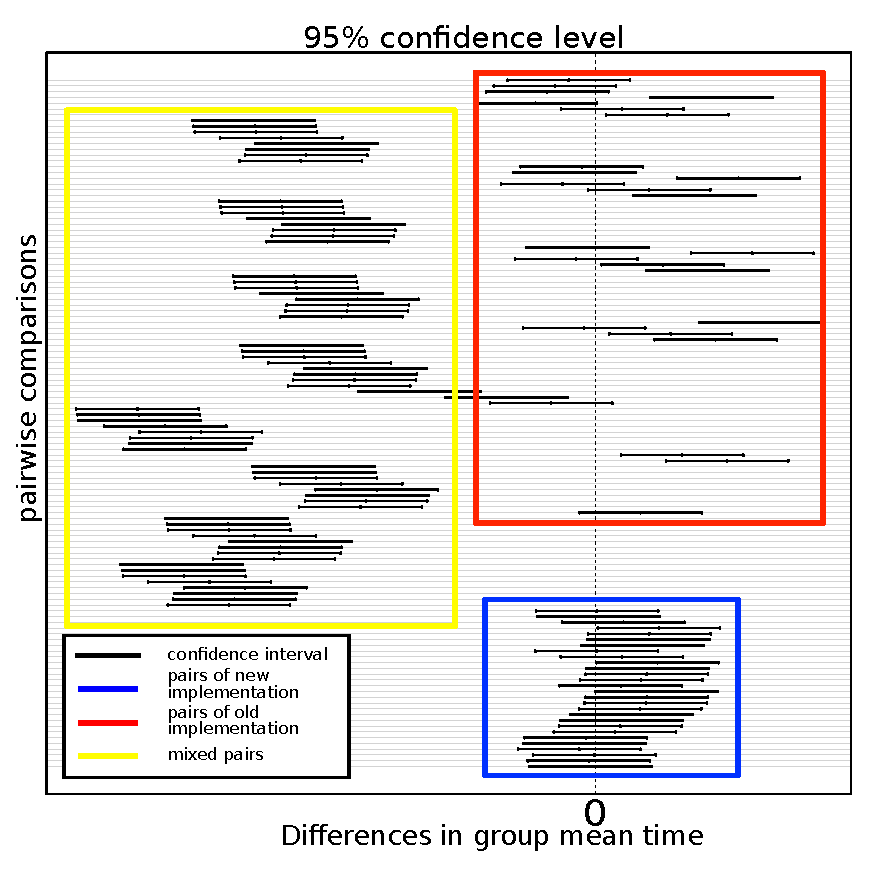
\includegraphics[width=0.4\textwidth]{images/tukey}
        \end{tikzfigure}
    }
    \block{Conclusion}{
        Obtained results allowed us
        to conclude that
        the developed approach
        do not lead to significant increase
        in RAM allocation thus making
        it possible to use
        more complex objective functions.
        An improved DEEP method ready
        to be used as the global optimizer
        in the field of systems biology
        and bioinformatics.
    }
    \column{0.55}
    \block{Trajectory segmentation task}
    {
        \begin{tikzfigure}
            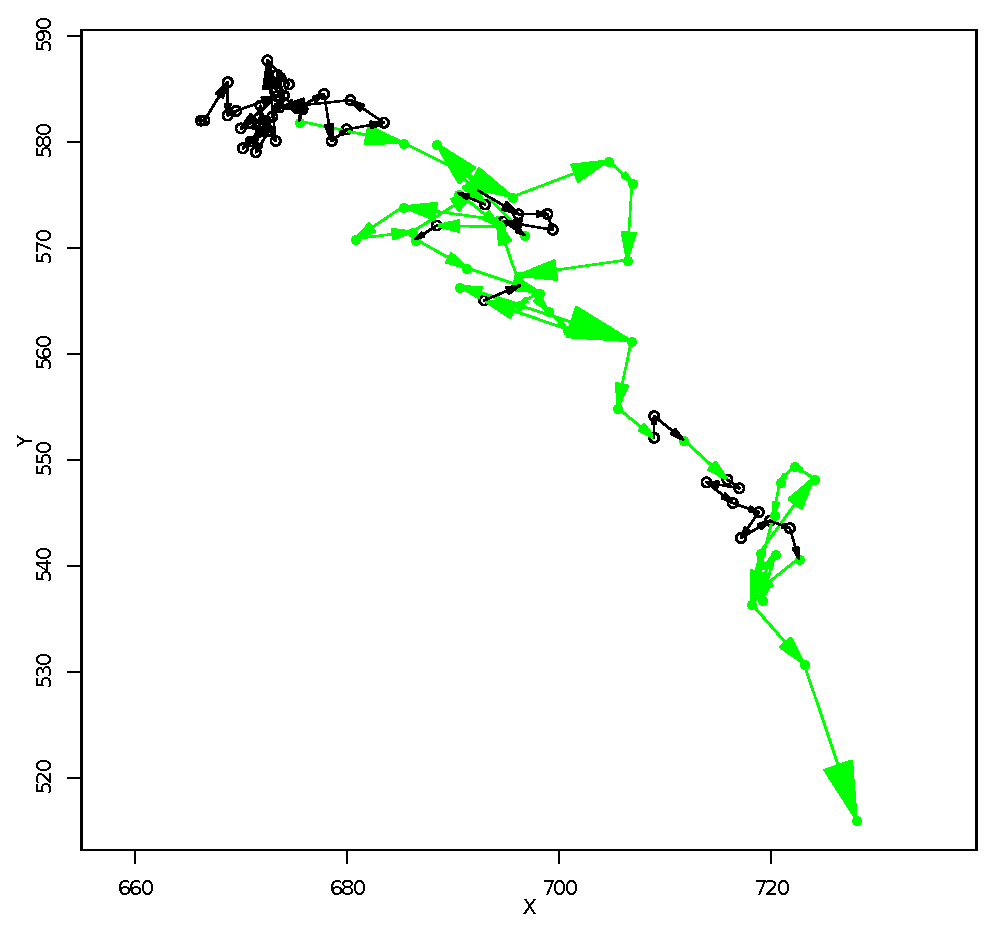
\includegraphics[width=0.3\textwidth]{images/track}
        \end{tikzfigure}
    }
    \block{Comparison of optimization}
    {
        \begin{tikzfigure}
            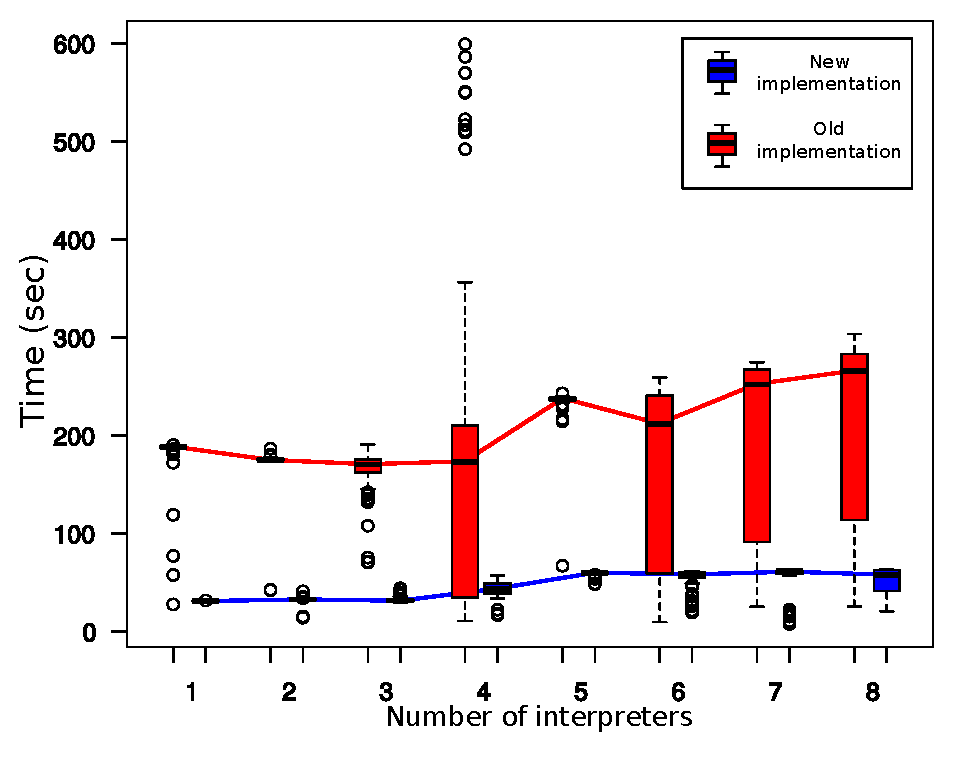
\includegraphics[width=0.45\textwidth]{images/m5}
        \end{tikzfigure}
    }
\end{columns}


\end{document}
